\documentclass[11pt]{article}

% --------------------------------------------------
% PACKAGES
% --------------------------------------------------
\usepackage[a4paper,margin=1in]{geometry}
\usepackage{amsmath, amssymb, amsthm}
\usepackage{mathtools}
\usepackage{enumitem}
\usepackage{graphicx}
\usepackage{hyperref}
\usepackage{booktabs}
\usepackage{float}

% --------------------------------------------------
% CUSTOM SETTINGS
% --------------------------------------------------
\setlength{\parindent}{0pt}
\setlength{\parskip}{6pt}

\hypersetup{
    colorlinks=true,
    linkcolor=blue,
    urlcolor=blue
}

% --------------------------------------------------
% TITLE
% --------------------------------------------------
\title{Homework 2 \\ \large Forecasting and Nowcasting with Text as Data}
\author{Tizian Schenk · Eric Gutiérrez}
\date{\today}

% --------------------------------------------------
\begin{document}
\maketitle
\hrule
\vspace{1em}

% --------------------------------------------------
% INSTRUCTIONS FOR STRUCTURE
% --------------------------------------------------
\textit{Please refer to the notebook forecasting-h2\_schenk\_gutierrez.ipynb for the code implementation.}

\vspace{12pt}

\section*{Part I}

\subsection*{1. Dataset Construction}

Figure~\ref{fig:1} displays four panels with the raw data series that will
be used throughout this project. Notice how the plots are identical to those
provided in the assignment, which validates that the downloaded and filtered
data is as required.

\begin{figure}[H]
    \centering
    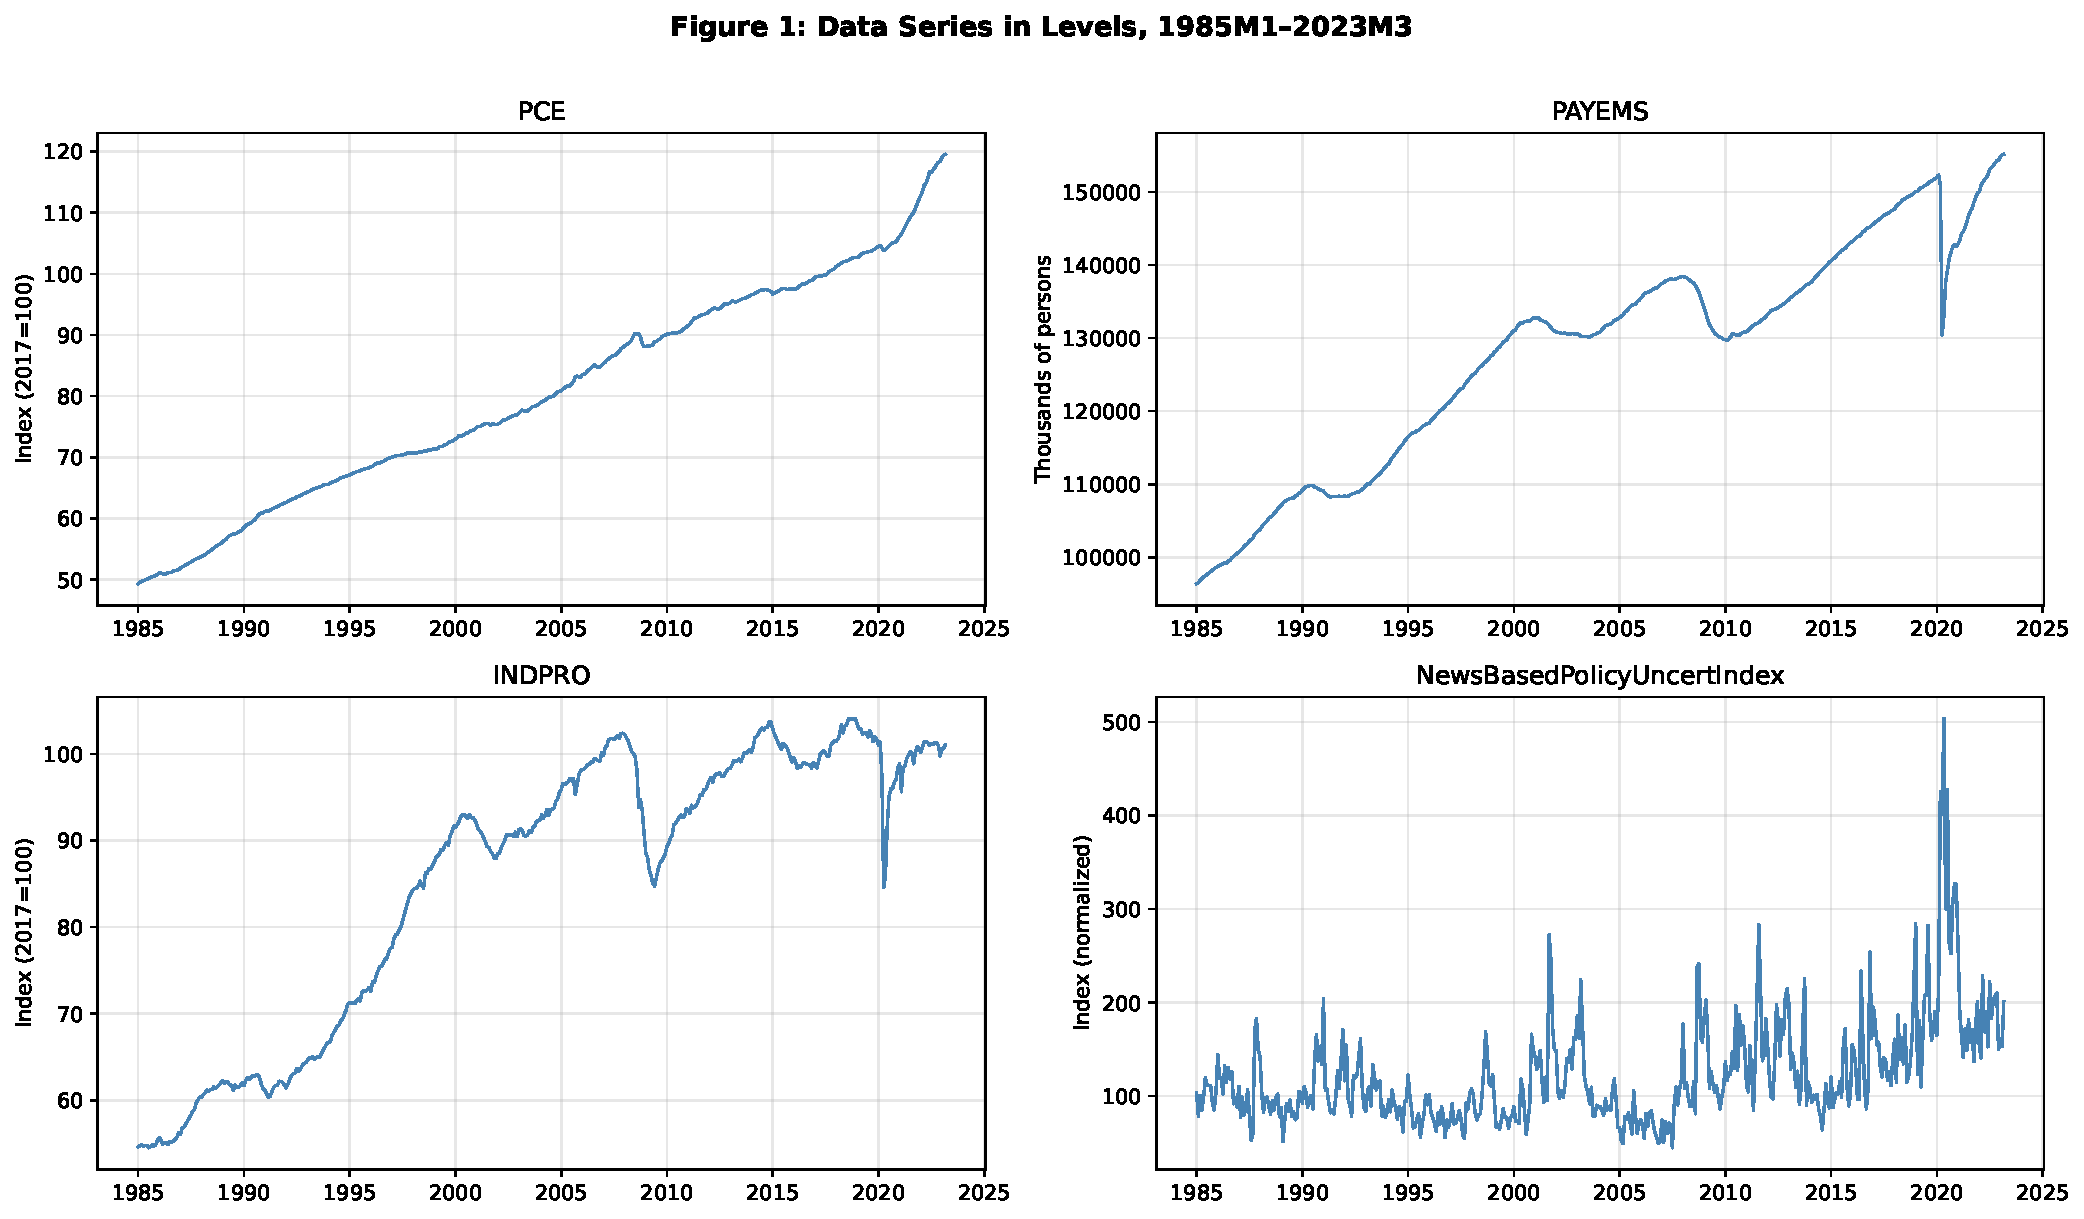
\includegraphics[width=1\textwidth]{../output/figure1_data_levels.pdf}
    \caption{Data Series in Levels.}
    {\small \textit{Note: The four panels show the raw data series in levels, seasonally adjusted, 
    downloaded from FRED (PAYEMS, PCEPI, INDPRO) and policyuncertainty.com (EPU). Sample: 1985M1-2023M3.}}
    \label{fig:1}
\end{figure}

\subsection*{2. VAR Estimation}

The reduced-form VAR(1) estimates (Tables \ref{tab:var_epu}, \ref{tab:var_payems}, \ref{tab:var_indpro}, and \ref{tab:var_pcepi}) 
reveal a clear and coherent dynamic structure across the four macroeconomic variables. Each series is strongly influenced by its 
own past value, with the largest autoregressive coefficients found in EPU (0.641) and PAYEMS\_g (0.679). These values indicate that 
uncertainty and employment growth adjust slowly over time, so shocks to these variables persist for many months. In contrast, 
industrial production growth shows almost no persistence (0.073), which implies that deviations in INDPRO\_g tend to dissipate quickly. 
Inflation, measured by PCEPI\_g, displays moderate persistence (0.404), consistent with the well‑known stickiness of monthly price changes.

\begin{figure}[H]
\centering

%------------------ Row 1 ------------------%
\begin{minipage}{0.48\textwidth}
\begin{table}[H]
\centering
\caption{EPU Equation}
\label{tab:var_epu}
\begin{tabular}{lccc}
\hline
Variable & Coef. & Std.Err. & t-stat \\
\hline
const        & 46.0666  & 5.3457  & 8.617 \\
L1.EPU       & 0.6408   & 0.0380  & 16.876 \\
L1.PAYEMS\_g & -19.3130 & 11.3933 & -1.695 \\
L1.INDPRO\_g & -3.5399  & 2.8356  & -1.248 \\
L1.PCEPI\_g  & -13.2245 & 8.3582  & -1.582 \\
\hline
\end{tabular}
\begin{flushleft}
\footnotesize \textit{Note: Reduced-form OLS estimates for the EPU equation.}
\end{flushleft}
\end{table}
\end{minipage}
\hfill
\begin{minipage}{0.48\textwidth}
\begin{table}[H]
\centering
\caption{PAYEMS\_g Equation}
\label{tab:var_payems}
\begin{tabular}{lccc}
\hline
Variable & Coef. & Std.Err. & t-stat \\
\hline
const        & 0.0579    & 0.0179   & 3.238 \\
L1.EPU       & -0.000278 & 0.000127 & -2.191 \\
L1.PAYEMS\_g & 0.6792    & 0.0381   & 17.831 \\
L1.INDPRO\_g & 0.0168    & 0.0095   & 1.775 \\
L1.PCEPI\_g  & 0.0331    & 0.0279   & 1.186 \\
\hline
\end{tabular}
\begin{flushleft}
\footnotesize \textit{Note: Employment growth equation. Lagged EPU is negative and significant.}
\end{flushleft}
\end{table}
\end{minipage}

\vspace{1em}

%------------------ Row 2 ------------------%
\begin{minipage}{0.48\textwidth}
\begin{table}[H]
\centering
\caption{INDPRO\_g Equation}
\label{tab:var_indpro}
\begin{tabular}{lccc}
\hline
Variable & Coef. & Std.Err. & t-stat \\
\hline
const        & 0.1108    & 0.0970   & 1.143 \\
L1.EPU       & -0.001359 & 0.000689 & -1.974 \\
L1.PAYEMS\_g & 0.9249    & 0.2066   & 4.476 \\
L1.INDPRO\_g & 0.0731    & 0.0514   & 1.422 \\
L1.PCEPI\_g  & 0.4582    & 0.1516   & 3.023 \\
\hline
\end{tabular}
\begin{flushleft}
\footnotesize \textit{Note: Industrial production growth equation. Employment growth has a strong effect.}
\end{flushleft}
\end{table}
\end{minipage}
\hfill
\begin{minipage}{0.48\textwidth}
\begin{table}[H]
\centering
\caption{PCEPI\_g Equation}
\label{tab:var_pcepi}
\begin{tabular}{lccc}
\hline
Variable & Coef. & Std.Err. & t-stat \\
\hline
const        & 0.1682    & 0.0287   & 5.857 \\
L1.EPU       & -0.000578 & 0.000204 & -2.834 \\
L1.PAYEMS\_g & 0.0209    & 0.0612   & 0.342 \\
L1.INDPRO\_g & 0.0093    & 0.0152   & 0.610 \\
L1.PCEPI\_g  & 0.4037    & 0.0449   & 8.992 \\
\hline
\end{tabular}
\begin{flushleft}
\footnotesize \textit{Note: Inflation equation. Inflation is persistent and responds negatively to lagged EPU.}
\end{flushleft}
\end{table}
\end{minipage}

\end{figure}

The lagged EPU term plays a central role in the system. It enters negatively and significantly in all three real‑activity equations, 
indicating that higher uncertainty in the previous month predicts lower employment growth, lower industrial production growth, and 
lower inflation. Although the month‑to‑month magnitudes are small, they accumulate through the VAR dynamics, meaning that an initial 
rise in uncertainty propagates forward and affects the economy over several periods. The cross‑variable interactions also reveal 
meaningful structure: lagged employment growth strongly predicts industrial production growth, while the reverse is not true, 
suggesting that labor market conditions tend to lead output at the monthly frequency. Lagged inflation also helps explain industrial 
production growth, consistent with the idea that stronger demand pressures translate into higher production. These relationships are 
reduced‑form correlations rather than causal effects, which is why structural identification is required before drawing economic 
conclusions about the impact of uncertainty shocks.

{\small
\begin{align}
\text{EPU}_t
&= 46.0666
+ 0.6408\, \text{EPU}_{t-1}
- 19.3130\, \text{PAYEMS\_g}_{t-1} \nonumber \\
&\quad
- 3.5399\, \text{INDPRO\_g}_{t-1}
- 13.2245\, \text{PCEPI\_g}_{t-1}
+ u^{EPU}_t
\end{align}

\begin{align}
\text{PAYEMS\_g}_t
&= 0.0579
- 0.000278\, \text{EPU}_{t-1}
+ 0.6792\, \text{PAYEMS\_g}_{t-1} \nonumber \\
&\quad
+ 0.0168\, \text{INDPRO\_g}_{t-1}
+ 0.0331\, \text{PCEPI\_g}_{t-1}
+ u^{PAY}_t
\end{align}

\begin{align}
\text{INDPRO\_g}_t
&= 0.1108
- 0.001359\, \text{EPU}_{t-1}
+ 0.9249\, \text{PAYEMS\_g}_{t-1} \nonumber \\
&\quad
+ 0.0731\, \text{INDPRO\_g}_{t-1}
+ 0.4582\, \text{PCEPI\_g}_{t-1}
+ u^{IND}_t
\end{align}

\begin{align}
\text{PCEPI\_g}_t
&= 0.1682
- 0.000578\, \text{EPU}_{t-1}
+ 0.0209\, \text{PAYEMS\_g}_{t-1} \nonumber \\
&\quad
+ 0.0093\, \text{INDPRO\_g}_{t-1}
+ 0.4037\, \text{PCEPI\_g}_{t-1}
+ u^{PCE}_t
\end{align}
}

The residual variances detailed in Table \ref{tab:resid_corr} show that EPU is by far the noisiest series, with a standard deviation of 31.05, 
while employment growth is the most predictable. Off‑diagonal correlations are small, indicating limited 
contemporaneous co‑movement. The strongest is between PAYEMS\_g and INDPRO\_g (0.32), suggesting shared 
shocks. These correlations matter because the structural impact matrix is obtained by applying the Cholesky 
decomposition to this residual covariance structure.


\begin{table}[H]
\centering
\caption{Correlation Matrix of Reduced-Form Residuals}
\label{tab:resid_corr}
\begin{tabular}{lcccc}
\hline
            & EPU      & PAYEMS\_g & INDPRO\_g & PCEPI\_g \\
\hline
EPU         & 1.000000 & -0.056580 & -0.054108 & -0.018936 \\
PAYEMS\_g   & -0.056580 & 1.000000 & 0.319911  & 0.078671  \\
INDPRO\_g   & -0.054108 & 0.319911  & 1.000000 & -0.024266 \\
PCEPI\_g    & -0.018936 & 0.078671  & -0.024266 & 1.000000 \\
\hline
\end{tabular}
\begin{flushleft}
\footnotesize \textit{Note: The table reports the contemporaneous correlations among the reduced-form VAR(1) residuals. Diagonal elements equal one by construction. Off-diagonal values measure the degree of residual co-movement not explained by lagged variables.}
\end{flushleft}
\end{table}


\subsection*{3. Impulse Response Function Estimation}

The plots displayed in Figure~\ref{fig:2} show that a shock to economic policy uncertainty causes a clear drop in both employment and industrial 
production growth. This confirms the classic "wait-and-see" theory, which suggests that firms pause their production and 
hiring when they face unpredictable policy environments. It is worth noting that neither variable shows a statistically 
significant reaction in the very first month. This validates our decision to place the uncertainty index first in our model, 
as it confirms that the real economy takes at least a month to process and react to policy news. After that initial delay, a 
single standard deviation shock pushes both growth rates down for about a full year. Both series then begin a smooth recovery 
and return to their normal baseline levels roughly 18 to 24 months later. Finally, our simple model produces a slow and steady 
recovery instead of the sharp bounce-back that some theories predict. Because this negative effect lingers for so long, it 
perfectly explains why our later forecasts that focus on election periods look so different from our standard baseline predictions

\begin{figure}[H]
    \centering
    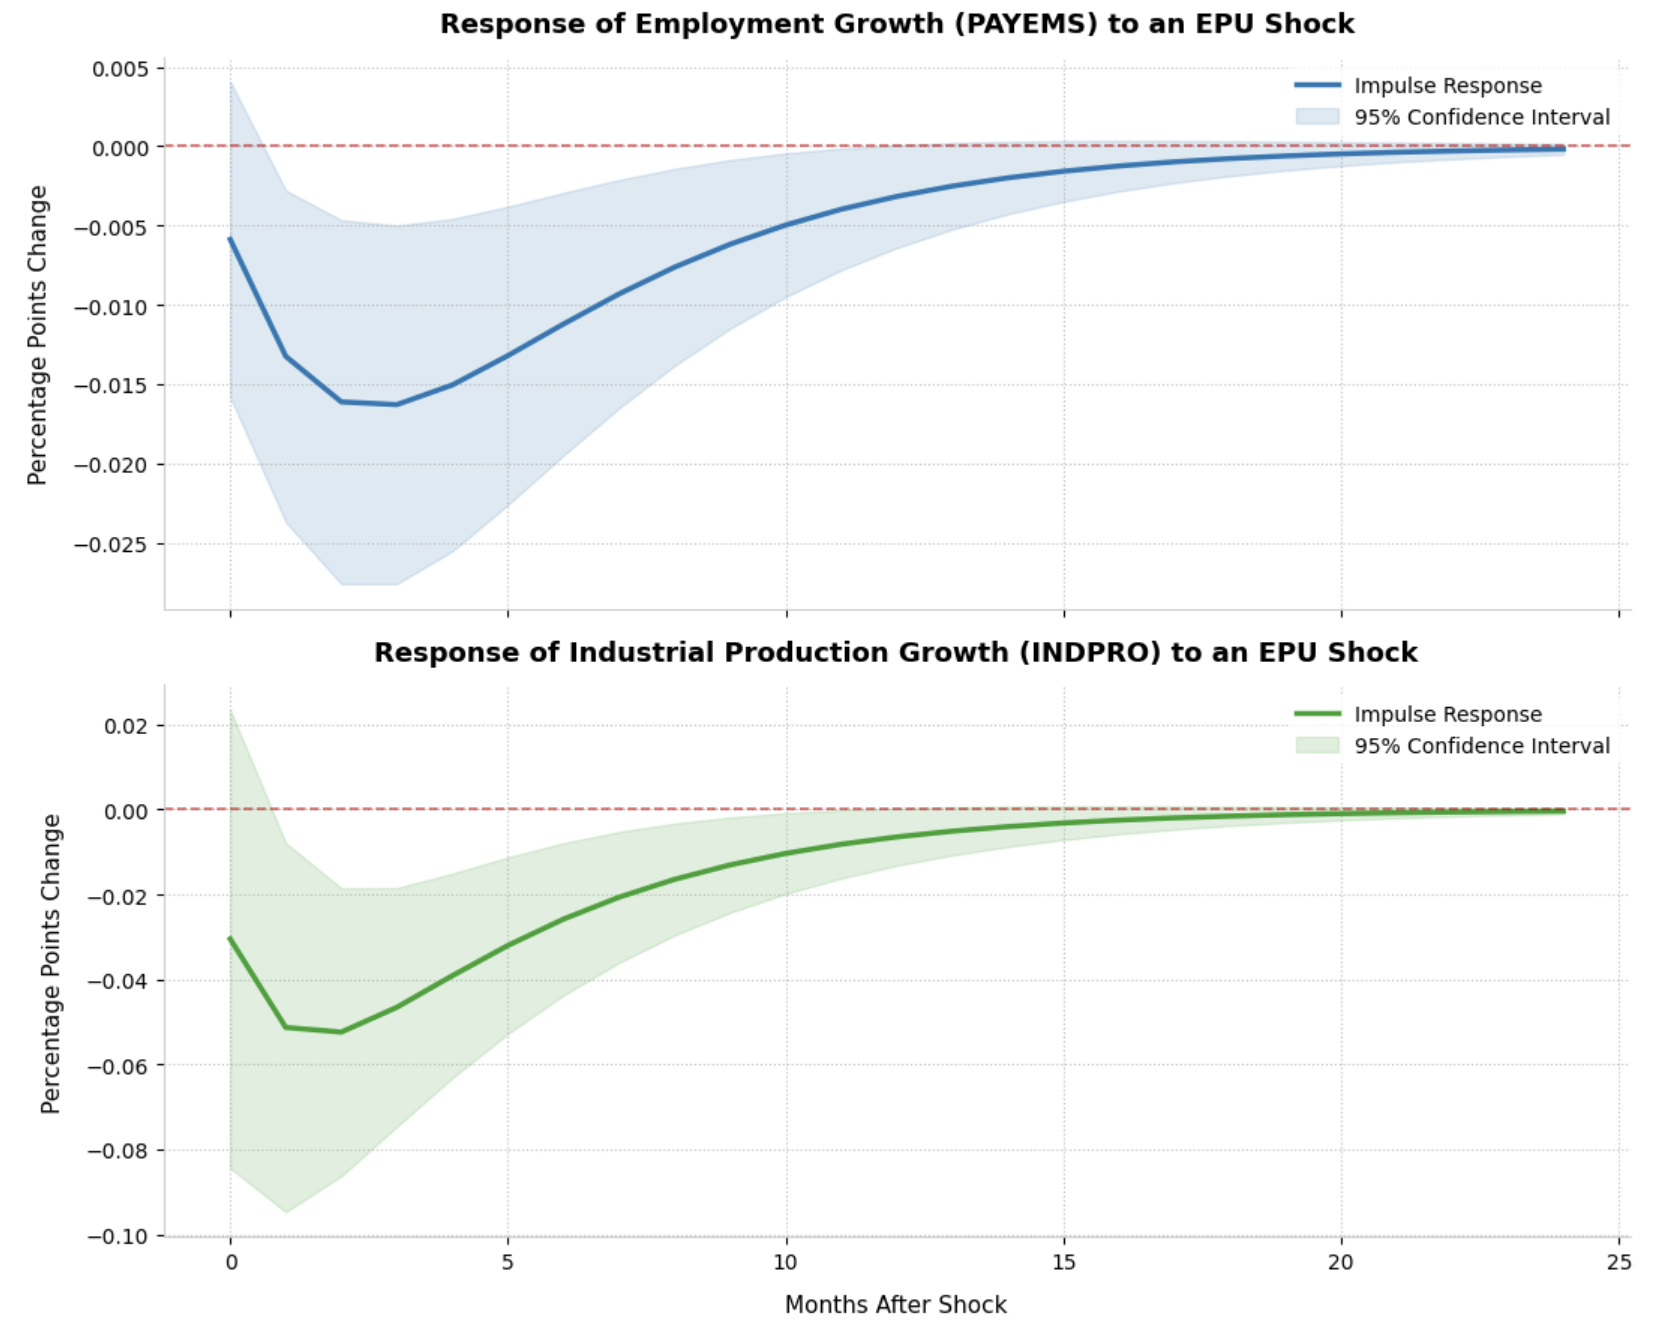
\includegraphics[width=.9\textwidth]{../output/fig2_erics.png}
    \caption{Impulse Response Function for a shock to the EPU for PAYEMS and INDPRO.}
    {\small \textit{Note: The two panels show the orthogonalized impulse response functions of month-on-month 
    employment growth (PAYEMS, top panel) and industrial production growth (INDPRO, bottom panel) to a one-standard-deviation 
    structural shock to the Economic Policy Uncertainty (EPU) index. The solid lines indicate the point estimates, while the 
    shaded regions represent the 95\% confidence bands. Shocks are identified via a Cholesky decomposition where the EPU index is ordered first.}}
    \label{fig:2}
\end{figure}

\section*{Part II}

\subsection*{1. Unconditional Forecasting}

Figure~\ref{fig:3} visually confirms the trajectory of our unconditional forecasts, with the left panel showing that employment 
growth remains strictly positive throughout the entire 12-month horizon. The forecast begins with a nearly flat path between 
March and May 2023, which reflects a tug-of-war between the lingering negative drag of the high uncertainty shock and the 
underlying positive momentum of the labor market. From June 2023 onward, as the policy uncertainty naturally fades, 
employment growth smoothly and steadily accelerates toward its historical long-run mean. Overall, the model predicts a 
resilient labor market with no recessionary conditions over the coming year.


In contrast, the right panel illustrates a much more dramatic, U-shaped recovery for industrial production growth. The 
model predicts an immediate and sharp drop into a contraction zone, with growth turning slightly negative from April through 
June 2023 as the high uncertainty forces a temporary halt in manufacturing and output. However, after hitting its trough, 
industrial production turns positive in July 2023 and climbs steadily for the remainder of the forecast horizon. Ultimately, 
both variables illustrate the underlying mechanics of our model, as they spend the year smoothly converging back toward their 
respective long-run historical averages.

\begin{figure}[H]
    \centering
    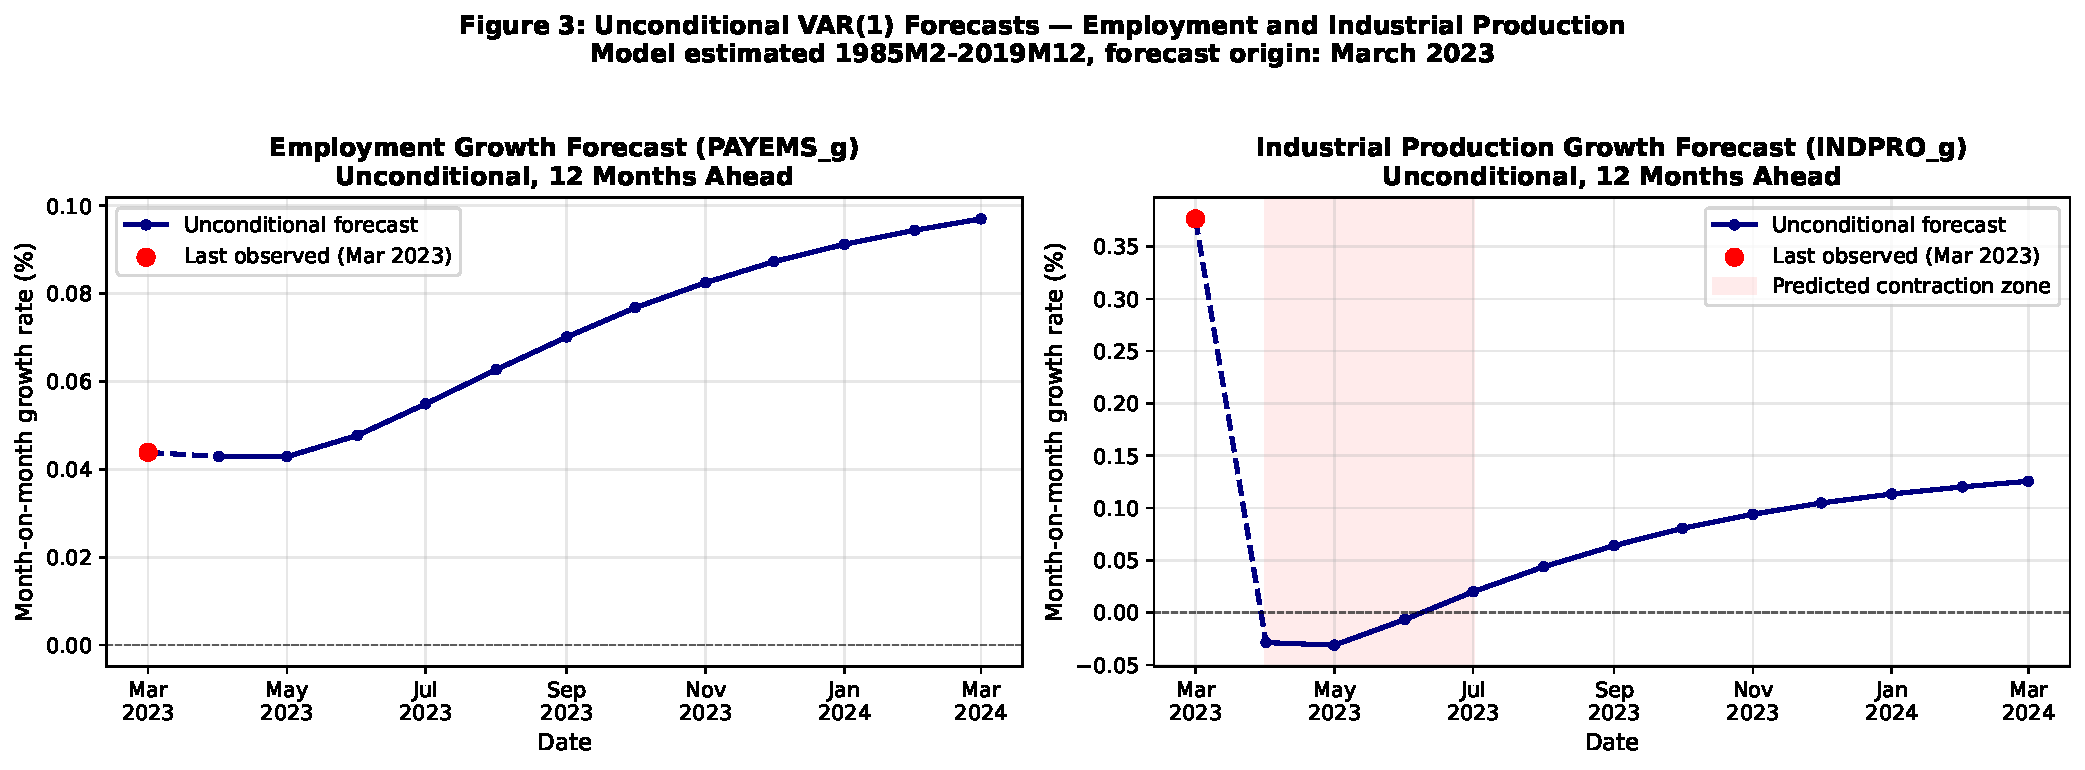
\includegraphics[width=1\textwidth]{../output/figure3_unconditional_forecast.pdf}
    \caption{Unconditional forecasts for month-on-month PAYEMS and INDPRO growth.}
    {\small \textit{Note: The two panels present the unconditional 12-month-ahead forecasts for month-on-month 
    employment growth (left panel) and industrial production growth (right panel). The underlying VAR(1) model 
    is estimated over the sample period 1985M2--2019M12. The solid red dots indicate the forecast origin at the 
    last observed data point in March 2023. The shaded region in the right panel highlights a predicted contraction 
    zone where industrial production growth is forecasted to fall below zero.}}
    \label{fig:3}
\end{figure}

\subsection*{2. Structural Conditional Forecasting}

\begin{figure}[H]
    \centering
    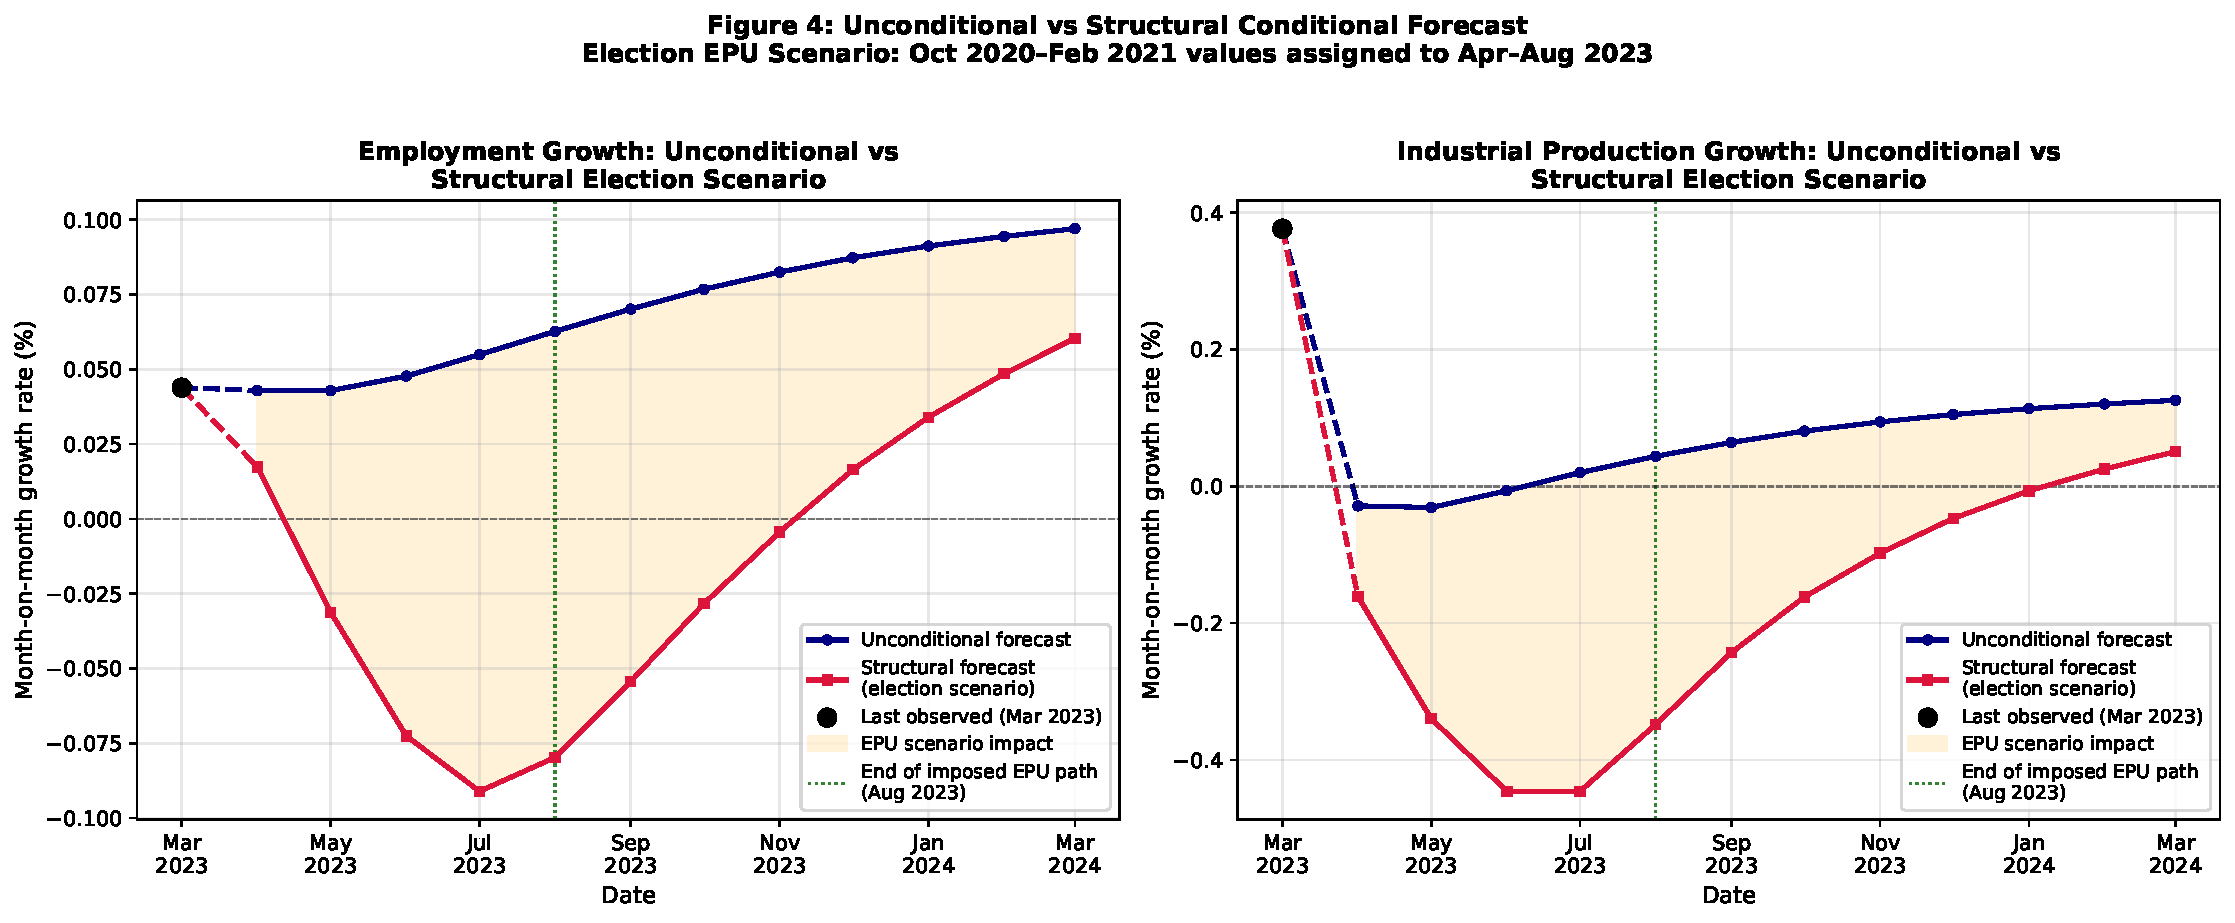
\includegraphics[width=1\textwidth]{../output/figure4_structural_vs_unconditional.pdf}
    \caption{Comparison of the unconditional and structural conditional forecasts for month-on-month PAYEMS and INDPRO.}
    {\small \textit{Note: The two panels compare the unconditional 12-month-ahead forecasts (blue lines) with the structural 
    conditional forecasts (red lines) for month-on-month employment growth (left panel) and industrial production growth (right panel). 
    The conditional "election scenario" forces the Economic Policy Uncertainty (EPU) index from April to August 2023 to mirror the exact 
    historical path observed during the previous U.S. national election period (October 2020 to February 2021). The shaded regions 
    illustrate the macroeconomic impact of this heightened uncertainty relative to the unconditional baseline. The vertical dotted 
    lines mark August 2023, the end of the imposed EPU path.}}
    \label{fig:4}
\end{figure}

\subsection*{3. Forecast Comparison}

The forecasts from parts (1) and (2) are substantially different, as can be seen in Figure~\ref{fig:4}. The unconditional forecast predicts 
a slow but steady labor market recovery with strictly positive employment growth and a mild, brief contraction in industrial production that 
quickly turns positive. In contrast, the structural scenario, which simulates the uncertainty of a national election, projects a deep and 
prolonged contraction across both variables. Employment growth turns negative for over half a year, and the drop in industrial production 
is roughly 15 times larger than in the unconditional baseline. This severe divergence occurs because the unconditional model expects 
uncertainty to smoothly fade away, whereas the structural scenario forces the model to absorb massive, unexpected spikes in uncertainty 
(representing the election panic). These shocks act as a heavy drag on the real economy, and because hiring and production are persistent 
processes, the damage lingers for months even after the election uncertainty has officially ended.

This structural forecast is fundamentally a causal "what-if" scenario. It doesn't just ask what happens if the EPU index goes up; it 
specifically asks what happens if the EPU index goes up because of an isolated policy shock. By using the Cholesky matrix to isolate this 
exact type of shock, the model ensures that the resulting economic damage isn't just statistical noise, but rather the direct cause-and-effect 
consequence of the election uncertainty rippling through the system.

\subsection*{4. Shortcomings}

The entire structural analysis relies on fragile identification assumptions, specifically the choice to place the policy uncertainty index 
first in the model. This mathematically forces the assumption that news coverage of uncertainty does not react to a sudden drop in industrial
production within the same month. In reality, journalists write about economic downturns exactly as they happen. Because our model ignores this 
potential reverse causality, it might be mixing up causes and effects, which ultimately biases the results of the structural forecast.

Additionally, the model relies on outdated estimation data, having been trained entirely on historical figures from 1985 to 2019 to forecast 
the economy in 2023. The post-pandemic economy experienced massive structural shifts, including supply chain breakdowns, unprecedented labor 
market reallocation, and historically high inflation. Because the model learned the economic relationships of a completely different era, 
applying those old rules to forecast a new economic regime might lead to systematically inaccurate predictions.

Finally, the uncertainty index itself conflates several different economic measures by bundling media sentiment, expiring tax codes, and 
disagreements among professional forecasters into a single number. When the forecast is forced to mimic the uncertainty of the 2020 election, 
it implicitly assumes that all three of these distinct components would repeat their exact past behavior. The index also broadly mixes general 
political anxiety with specific economic policy uncertainty, meaning the simulated shock is likely artificially exaggerated and lacks the 
precision needed for highly accurate scenario analysis


\end{document}